\documentclass[12pt]{report}
\usepackage[T1]{fontenc}
\usepackage[utf8]{inputenc}
\usepackage{lmodern, textcomp} %textcomp for usage of euro currency symbol
\usepackage{listings}
\usepackage[margin=1in]{geometry}
\usepackage{csquotes}
\usepackage[english]{babel}
\usepackage{color}
\usepackage{xcolor} %for more colours to use in hyperref
\usepackage{amsmath}
\usepackage{makecell} %for resizing hline
\usepackage{float}
\usepackage{graphicx} %for pictures
\graphicspath{ {figures/} }
\usepackage[
    backend=biber,
    style=numeric,
    sorting=none
    ]{biblatex}
\addbibresource{ref.bib}

\usepackage{hyperref}
\hypersetup{
    colorlinks=true, %set true if you want colored links
    linkcolor={red!50!black},
    citecolor={blue!50!black},
    urlcolor={blue!80!black}
    }
    
\usepackage{listings}
\usepackage{color}


\usepackage{graphicx}
\usepackage{caption}
\usepackage{subcaption}

\definecolor{mygreen}{rgb}{0,0.6,0}
\definecolor{mygray}{rgb}{0.5,0.5,0.5}
\definecolor{mymauve}{rgb}{0.58,0,0.82}

\lstset{ %
  backgroundcolor=\color{white},   % choose the background color; you must add \usepackage{color} or \usepackage{xcolor}; should come as last argument
  basicstyle=\footnotesize,        % the size of the fonts that are used for the code
  breakatwhitespace=false,         % sets if automatic breaks should only happen at whitespace
  breaklines=true,                 % sets automatic line breaking
  captionpos=b,                    % sets the caption-position to bottom
  commentstyle=\color{mygreen},    % comment style
  deletekeywords={...},            % if you want to delete keywords from the given language
  escapeinside={\%*}{*)},          % if you want to add LaTeX within your code
  extendedchars=true,              % lets you use non-ASCII characters; for 8-bits encodings only, does not work with UTF-8
  frame=single,	                   % adds a frame around the code
  keepspaces=true,                 % keeps spaces in text, useful for keeping indentation of code (possibly needs columns=flexible)
  keywordstyle=\color{blue},       % keyword style
  language=Octave,                 % the language of the code
  morekeywords={*,...},           % if you want to add more keywords to the set
  numbers=left,                    % where to put the line-numbers; possible values are (none, left, right)
  numbersep=5pt,                   % how far the line-numbers are from the code
  numberstyle=\tiny\color{mygray}, % the style that is used for the line-numbers
  rulecolor=\color{black},         % if not set, the frame-color may be changed on line-breaks within not-black text (e.g. comments (green here))
  showspaces=false,                % show spaces everywhere adding particular underscores; it overrides 'showstringspaces'
  showstringspaces=false,          % underline spaces within strings only
  showtabs=false,                  % show tabs within strings adding particular underscores
  stepnumber=2,                    % the step between two line-numbers. If it's 1, each line will be numbered
  stringstyle=\color{mymauve},     % string literal style
  tabsize=2,	                   % sets default tabsize to 2 spaces
  title=\lstname                   % show the filename of files included with \lstinputlisting; also try caption instead of title
}

\usepackage{algorithm}
\usepackage[noend]{algpseudocode}
\makeatletter
\def\BState{\State\hskip-\ALG@thistlm}
\makeatother

\newcommand*\samethanks[1][\value{footnote}]{\footnotemark[#1]}

\title{\Large{\textbf{RegGAN Summary}}\\\Large{}}

\author{
    Ahmad Shayaan\\as5948
    } 

\date{
\{\href{mailto:ahmad.shayaan@columbia.edu}{\texttt{\small{ahmad.shayaan@columbia.edu}}}\}\texttt{\small{@columbia.edu}}\\
    Columbia University\\
    \today}



\usepackage[utf8]{inputenc}

% Default fixed font does not support bold face
\DeclareFixedFont{\ttb}{T1}{txtt}{bx}{n}{12} % for bold
\DeclareFixedFont{\ttm}{T1}{txtt}{m}{n}{12}  % for normal

% Custom colors
\usepackage{color}
\definecolor{deepblue}{rgb}{0,0,0.5}
\definecolor{deepred}{rgb}{0.6,0,0}
\definecolor{deepgreen}{rgb}{0,0.5,0}

\usepackage{listings}

% Python style for highlighting
\newcommand\pythonstyle{\lstset{
		language=Python,
		basicstyle=\ttm,
		otherkeywords={self},             % Add keywords here
		keywordstyle=\ttb\color{deepblue},
		emph={MyClass,__init__},          % Custom highlighting
		emphstyle=\ttb\color{deepred},    % Custom highlighting style
		stringstyle=\color{deepgreen},
		frame=tb,                         % Any extra options here
		showstringspaces=false            % 
	}}
	
	
	% Python environment
	\lstnewenvironment{python}[1][]
	{
		\pythonstyle
		\lstset{#1}
	}
	{}
	
	% Python for external files
	\newcommand\pythonexternal[2][]{{
			\pythonstyle
			\lstinputlisting[#1]{#2}}}
	
	% Python for inline
	\newcommand\pythoninline[1]{{\pythonstyle\lstinline!#1!}}

\begin{document}

\maketitle

\pagebreak


\section*{Conditional Deep Convolutional Generative Adversarial Networks}
We tired to use a Conditional Deep Convolutional Generative Adversarial
Networks (CDCGAN) to generate the images. CDCGAN are an extension of the vanilla
DCGAN in which both the discriminator and the generator are conditioned on some extra
information. CDCGAN have been successfully use to generate medical data \href{https://openreview.net/forum?id=B1ZZTfZAW}{link}

The conditioning of the model on the extra gives the model an initial starting point to generate data. It also gives the user more control on what type of data we want the mode to generate. We condition both the generator and the discriminator on the number of connected components we want the generated image to have. We hoped that conditioning the model on the number of connected components would provide the model with necessary information so as to generate images with the desired structure. However empirically we found that this is not the case, the model fails to sufficiently leverage the extra information provided.


The high level architecture of the CDCGAN is shown below.

\begin{figure}[H]
	\centering
	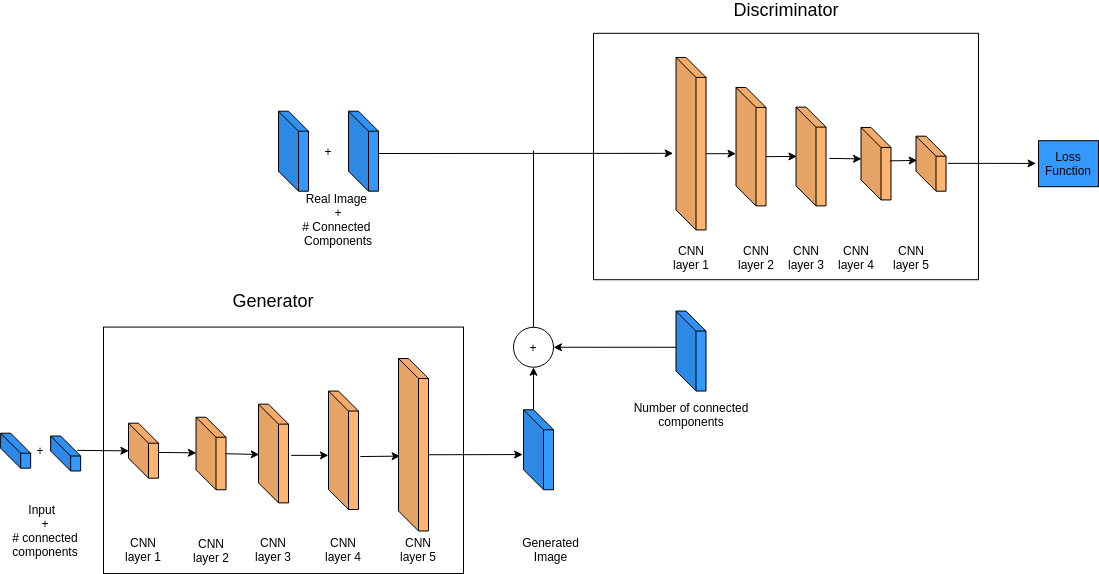
\includegraphics[scale=0.45]{CDCGAN}
\end{figure}


However the CDCGAN was not able to sufficiently capture the structures of the images and generated images as shown below.

\begin{figure}[H]
	\centering
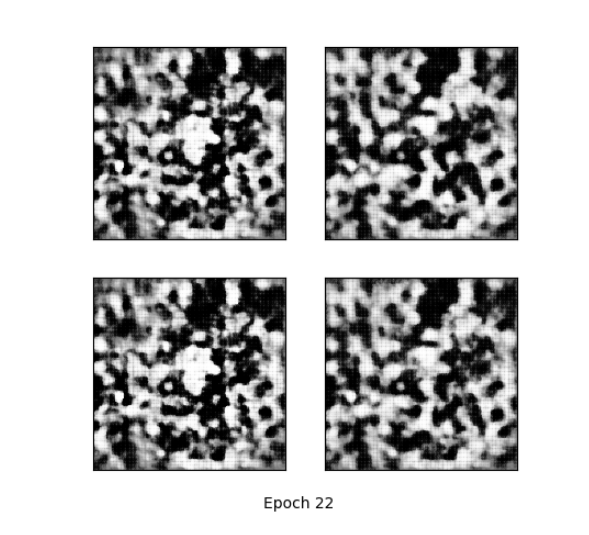
\includegraphics[scale=0.5]{cdcgan_result}
\end{figure}

It can be seen form the image above that the model is not able to use the extra information given by us.

\chapter*{RegGAN}

The RegGAN architecture consists of two discriminator and a single generator. The second discriminator is used to simulate the score function, which was designed by us. The first discriminator is used to differentiate between the images generated by the network and the ones from the dataset. The architecture can be seen below.

\begin{figure}[H]
	\centering
	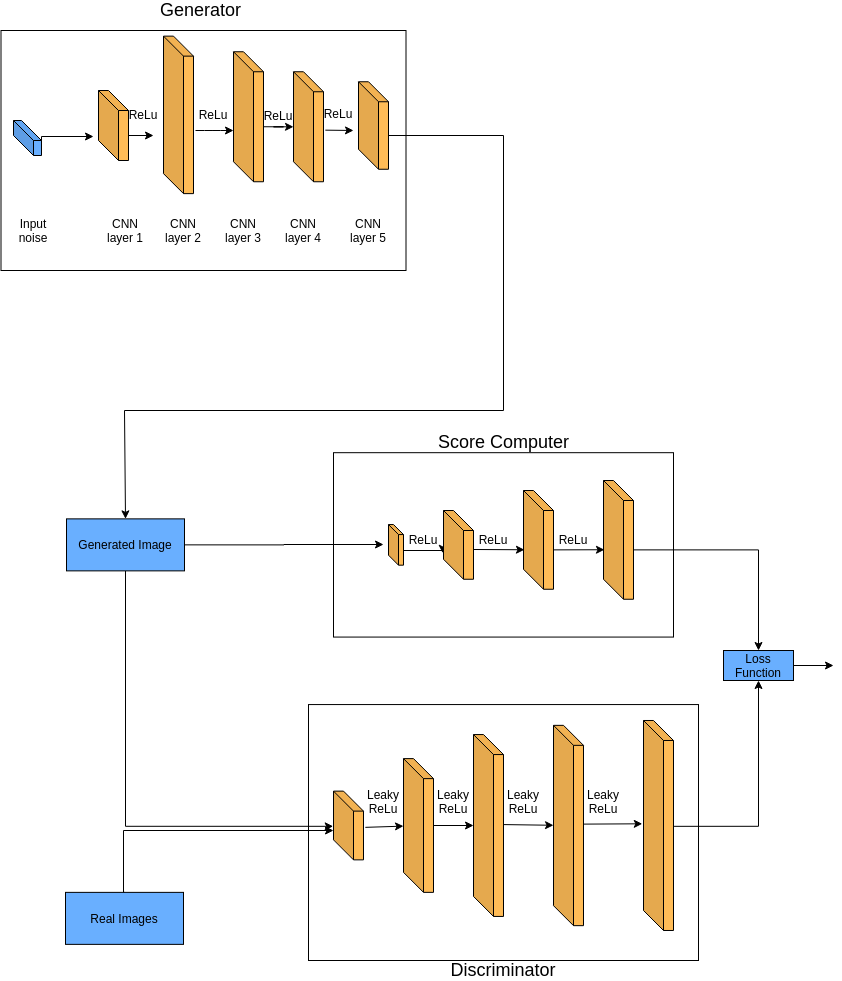
\includegraphics[scale=0.4]{RegGAN}
\end{figure} 

\section*{Pre-Training of Discriminator}

We pre-train the discriminator to learn the score function. This is done so that the second discriminator has a good starting point for the actual training of the network. The discriminator is a CNN with four layers. 
\\
During pre-training we feed in the images from the data set to the network. The outputs from the network are then compared to the actual scores given by the score function. The results from the training of the network are shown below. \emph{Pre-training helps the model to get to a good starting point}. Once the discriminator has converged close enough to the score function we freeze the weights of the model. We do so because we want to use the second discriminator, as a pseudo for the score function. For other applications, where the penalty function should evolve with the data the weights of the discriminator can evolve with the training of the generator.


\section*{Training RegGan}

The Generator and discriminator are also CNN both with 5 layers. We feed in noise to the generator and get outputs as images. These images are then fed into both the discriminators to compute the score and to compare it to the images of the actual data set. 

We have two ways in which we back-propagate. In the first one we freeze the weights of the second discriminator and the gradient is only propagated through the the generator and the first discriminator. In the second method we pass the gradient through the second discriminator as well. 


A sample of the images generated buy the network can be seen below. 

\begin{figure}[H]
	\centering
	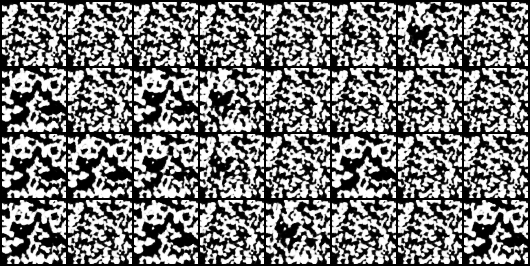
\includegraphics[scale=.6]{fake_samples_epoch_049}
\end{figure}

\end{document}